Die Summe der ersten $n$ ungeraden Zahlen ist $n^2$.
Beweisen Sie dies direkt, verwenden Sie dazu das folgende Diagramm:
\begin{center}
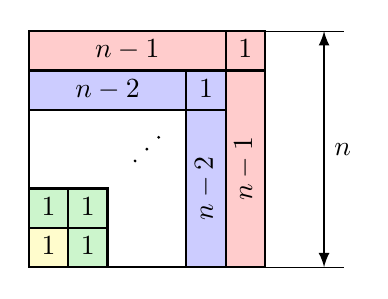
\begin{tikzpicture}[>=latex,thick]
\definecolor{darkgreen}{rgb}{0,0.8,0}
\def\h{0.5}
\def\punkt#1#2{({(#1)*\h},{(#2)*\h})}
\fill[color=red!20] \punkt{0}{0} rectangle \punkt{6}{6};
\fill[color=blue!20] \punkt{0}{0} rectangle \punkt{5}{5};
\fill[color=white] \punkt{0}{0} rectangle \punkt{4}{4};
\fill[color=darkgreen!20] \punkt{0}{0} rectangle \punkt{2}{2};
\fill[color=yellow!20] \punkt{0}{0} rectangle \punkt{1}{1};
\draw \punkt{0}{0} rectangle \punkt{6}{6};

\draw \punkt{0}{5} -- \punkt{6}{5};
\draw \punkt{5}{0} -- \punkt{5}{6};
\node at \punkt{5.5}{5.5} {$1\mathstrut$};
\node at \punkt{2.5}{5.5} {$n-1\mathstrut$};
\node at \punkt{5.5}{2.5} [rotate=90]{$n-1\mathstrut$};

\draw \punkt{0}{4} -- \punkt{5}{4};
\draw \punkt{4}{0} -- \punkt{4}{5};
\node at \punkt{4.5}{4.5} {$1\mathstrut$};
\node at \punkt{2.0}{4.5} {$n-2\mathstrut$};
\node at \punkt{4.5}{2.0} [rotate=90] {$n-2\mathstrut$};

\draw \punkt{0}{2} -- \punkt{2}{2} -- \punkt{2}{0};

\draw \punkt{1}{0} -- \punkt{1}{2};
\draw \punkt{0}{1} -- \punkt{2}{1};

\foreach \x in {-0.3,0,0.3}{
	\fill \punkt{3.0+\x}{3.0+\x} circle[radius=0.02];
}

\node at \punkt{1.5}{1.5} {$1\mathstrut$};
\node at \punkt{0.5}{1.5} {$1\mathstrut$};
\node at \punkt{1.5}{0.5} {$1\mathstrut$};

\draw \punkt{0}{1} -- \punkt{1}{1} -- \punkt{1}{0};
\node at \punkt{0.5}{0.5} {$1\mathstrut$};

\draw[line width=0.2pt] \punkt{6}{0} -- \punkt{8}{0};
\draw[line width=0.2pt] \punkt{6}{6} -- \punkt{8}{6};
\draw[<->] \punkt{7.5}{0} -- \punkt{7.5}{6};
\node at \punkt{7.5}{3.0} [right] {$n$};

\end{tikzpicture}
\end{center}

\begin{loesung}
Der obere und rechte Rand eines Quadrates mit Seitenlänge $n+1$ 
enthält $2n-1$ Felder.
Die $n$-te ungerade Zahl ist $2n-1$.
Die Summe der ersten $n$ ungeraden Zahlen ist daher der Flächeninhalt
eines Quadrates mit Seitenlänge, also
\[
\sum_{k=1}^{n} (2k-1)
=
n^2.
\qedhere
\]
\end{loesung}
